\documentclass{beamer}


\DeclareMathOperator*{\argmin}{arg\,min}
\DeclareMathOperator*{\argmax}{arg\,max}


\newcommand{\matrixl}{\left|\left|}
\newcommand{\matrixr}{\right|\right|}

\newcommand{\sign}{\mbox{sign}\,}
\newcommand{\F}{\mathcal{F}}
\newcommand{\Hh}{\mathcal{H}}
\newcommand{\R}{\mathbb{R}}
\newcommand{\E}{\mathbb{E}}
\newcommand{\N}{\mathbb{N}}
\newcommand{\Be}{\mbox{Be}}
\newcommand{\Reg}{\mbox{Regret}}
\newcommand{\dkl}{d_{\mbox{\tiny KL}}}
\newcommand{\Ss}{\mathcal{S}}
\newcommand{\ltwo}{\log_2 }
\newcommand{\A}{\mathcal{A}}

% пустое слово
\def\eps{\varepsilon}

% регулярные языки
\def\eqdef{\overset{\mbox{\tiny def}}{=}}
\newcommand{\niton}{\not\owns}


\usepackage{amsmath}
\usepackage{wrapfig}
\usepackage{enumerate}
\usepackage[makeroom]{cancel}
\usepackage{multicol,multirow}
\usepackage{hyperref}
\usepackage{tabularx}
\usepackage{amsfonts}
\usepackage{amssymb}
\usepackage{amsmath}
\usepackage{amsthm}

\usepackage[utf8]{inputenc}
\usepackage[russian]{babel}
\usepackage{amsmath,mathrsfs,mathtext}
\usepackage{graphicx, epsfig}
\usetheme{Warsaw}%{Singapore}%{Warsaw}%{Warsaw}%{Darmstadt}
\usecolortheme{sidebartab}
\definecolor{beamer@blendedblue}{RGB}{100,30,100}
%----------------------------------------------------------------------------------------------------------
\title[\hbox to 56mm{Обучение с подкреплением  \hfill\insertframenumber\,/\,\inserttotalframenumber}]
{Нижние границы на сожаление\\ в обучении с подкреплением}
\author[Сергей Володин]{\large \\Сергей Володин}
\institute{\large МФТИ}

\date{По статье\\ {\em Ian Osband, Benjamin Van Roy. On Lower Bounds for\\ Regret in Reinforcement Learning}}
%-------------------------------------------------------
\begin{document}
%-------------------------------------------------------
\begin{frame}
\titlepage
\end{frame}
%-------------------------------------------------------
\begin{frame}{Обучение с подкреплением}
%Обучение с подкреплением: схема агент-среда, положение в других сферах
\centering Агент взаимодействует со средой:
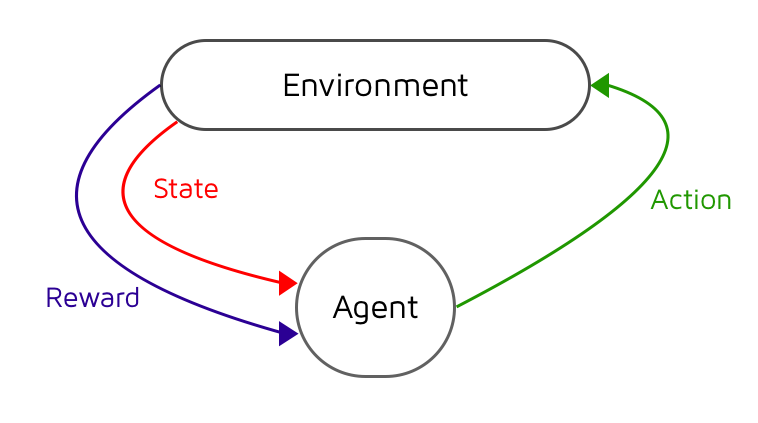
\includegraphics[width=200px]{RL.png}
\end{frame}

\begin{frame}{Определения}
%\theoremstyle{definition}
%\newtheorem{definition}{Определение}[section]
%\newtheorem{lemma}{Лемма}[section]
%\newtheorem{theorem}{Теорема}[section]
\begin{definition}
	
	ММПР~--- кортеж $(\mathcal{S}, \mathcal{A}, R, P)$, где
	\begin{enumerate}
		\item $\mathcal{S}=\{1,...,S\}$~--- состояния
		\item $\mathcal{A}=\{1,...,A\}$~--- действия
		\item $R(s,a)$~--- функция награды.
		\item $P(s,a)$~--- функция переходов.
	\end{enumerate}
\end{definition}
\begin{definition}
	$t\in\N$~--- время.
	\begin{enumerate}
		\item Агент получает состояние $s_t\in \Ss$
		\item Агент выбирает действие $a_t\in\A$
		\item Агент получает награду $r_t\sim R(s_t,a_t)\in[0,1]$
		\item Среда переходит в новое состояние $s_{t+1}\sim P(s_t,a_t)$
	\end{enumerate}
\end{definition}
\end{frame}

\begin{frame}{Определения}


\begin{definition}
	
	Политика $\mu$~--- отображение $\mu\colon \Ss\to\A$.
\end{definition}

\begin{definition}
Средняя награда:
	$$\lambda_{\mu}^M(s)=\lim\limits_{T\to\infty}\E_{M,\mu}\left[\frac{1}{T}\sum\limits_{t=1}^T\overline{r}(s_t,a_t)\big|s_1=s\right]$$
	
	$$\lambda_*^M(s)=\lambda_{\mu^M}^M(s)$$
	где $\overline{r}(s,a)=\E R(s,a)$ и $\mu^M\in\argmax\limits_{\mu}\lambda^M_{\mu}(s)$ 
\end{definition}

\end{frame}

\begin{frame}{Определения}

\begin{definition}
$\Hh_t=(s_1,a_1,r_1,...,s_{t-1},a_{t-1},r_{t-1})$~--- история для $t$.
\end{definition}

\begin{definition}
$\pi=\{\pi_t\big|t\in\N\}$~--- алгоритм RL, если $\pi_t$~--- функция, сопоставляющая истории $\Hh_t$ распределение над политиками
	
\end{definition}

\begin{definition}
Сожаление:
	$$\Reg(T,\pi,M,s)=T\lambda_*^M(s)-\sum\limits_{t=1}^Tr_t$$
\end{definition}
\end{frame}

\begin{frame}{Определения}
	
\begin{definition}
	Многорукий бандит $M$~--- ММПР с $S=1$
\end{definition}

\begin{theorem}
	Для любого $\pi$ существует функция награды $R$, такая что
	$$\E\Reg(T,\pi,M)\geqslant \frac{1}{24}\sqrt{AT}$$
\end{theorem}
\end{frame}


\end{document} 